\section{State composition: who writes the state}
\label{sec:composition}

Sections~\ref{sec:capability}--\ref{sec:economics} show that the damage comes
from discarded history, and that the agent pays for the loss by re-acquiring
the same information through its tools. This suggests a fix: if the state
already held the facts the agent keeps re-deriving, it would not need to
re-acquire them.

This section varies one thing: how much of the state the \emph{runtime}
writes on its own, without asking the model. That is a different axis from
the tail, and we report it separately because it answers a different
question. The tail axis asks how much history to keep. This axis asks, for a
fixed amount of history (none), who should produce the state that replaces
it.

% Adapted from the repository's original state-ownership diagram.
\begin{figure}[tbp]
\centering
\resizebox{\linewidth}{!}{%
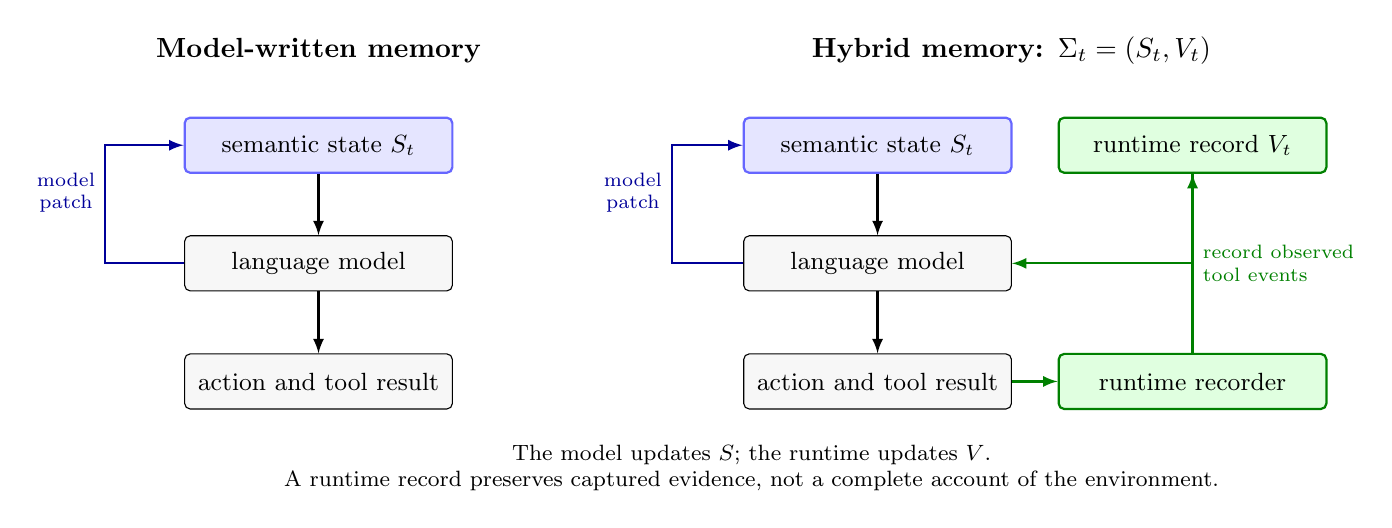
\begin{tikzpicture}[
font=\small,
box/.style={draw,rounded corners=2pt,minimum width=3.4cm,minimum height=.7cm,align=center,inner sep=3pt},
state/.style={box,fill=blue!10,draw=blue!60,thick},
record/.style={box,fill=green!12,draw=green!50!black,thick},
plain/.style={box,fill=black!3},
arr/.style={-latex,thick}]
\node[font=\bfseries] at (0,3.5) {Model-written memory};
\node[state] (s1) at (0,2.3) {semantic state $S_t$};
\node[plain] (m1) at (0,.8) {language model};
\node[plain] (a1) at (0,-.7) {action and tool result};
\draw[arr] (s1)--(m1);
\draw[arr] (m1)--(a1);
\draw[arr,blue!60!black] (m1.west)--++(-1,0)|-(s1.west)
node[pos=.3,left,font=\scriptsize,align=center]{model\\patch};
\begin{scope}[xshift=7.1cm]
\node[font=\bfseries] at (1.7,3.5) {Hybrid memory: $\Sigma_t=(S_t,V_t)$};
\node[state] (s2) at (0,2.3) {semantic state $S_t$};
\node[record] (v2) at (4,2.3) {runtime record $V_t$};
\node[plain] (m2) at (0,.8) {language model};
\node[plain] (a2) at (0,-.7) {action and tool result};
\node[record] (rec) at (4,-.7) {runtime recorder};
\draw[arr] (s2)--(m2);
\draw[arr,green!50!black] (v2.south)|-(m2.east);
\draw[arr] (m2)--(a2);
\draw[arr,blue!60!black] (m2.west)--++(-.9,0)|-(s2.west)
node[pos=.3,left,font=\scriptsize,align=center]{model\\patch};
\draw[arr,green!50!black] (a2)--(rec);
\draw[arr,green!50!black] (rec)--(v2)
node[midway,right,font=\scriptsize,align=left]{record observed\\tool events};
\end{scope}
\node[font=\footnotesize,align=center] at (5.5,-1.8)
{The model updates $S$; the runtime updates $V$.\\A runtime record preserves captured evidence, not a complete account of the environment.};
\end{tikzpicture}}
\caption{State ownership. Hybrid memory retains model-written semantic content and adds runtime-derived records. Recording an event does not establish that an extracted interpretation is correct or that all relevant events were captured.}
\label{fig:runtime-written}
\end{figure}


\subsection{The factor}

In \SkillState{} the state block is generated text: the model writes
$\Delta\Sigma_t$ in the same completion as its action
(Algorithm~\ref{alg:state}). \S\ref{sec:economics} gives two reasons this is
costly. First, maintaining the state is billed at the output tariff $\beta$,
the most expensive class in Eq.~\eqref{eq:cost}. Second, the model is free to
overwrite a fact it recorded earlier, and the original's own error taxonomy
attributes \SI{68}{\percent} of open-weight failures to exactly that
mistake\origin.

The alternative is to let the runtime record what already happened. A tool
result is an observed fact, not a claim: the runtime saw which files were
touched, which command ran, what it printed, and whether the tests passed.
Writing those facts into the state needs no generation, and the model cannot
overwrite them.

How much to record is the factor we vary here. The ladder adds one component
per rung:

\begin{center}
\begin{tabular}{@{}llp{0.52\linewidth}@{}}
\toprule
Rung & Adds & What the runtime writes \\
\midrule
v1 & files        & paths the agent has touched \\
v2 & + content    & per-file and global modification records \\
v3 & + commands   & normalised command records with their output \\
v4 & + diagnostics& compiler and linter output, structured \\
v5 & + environment& versions, paths, interpreter state \\
v6 & + tests      & test invocations and their results \\
v7 & + failures   & records of what was tried and did not work \\
\bottomrule
\end{tabular}
\end{center}

The tail is frozen at $\tailk{=}0$, and the schema is fixed at
\texttt{L2-semantic} in every cell, so no rung borrows an advantage from the
factors of \S\ref{sec:capability}. Neighbouring rungs differ by exactly one
component, and we check that invariant against the flags the conditions
actually emit before a cell runs, not against what we intended them to
emit\code.

\paragraph{Why this series needs its own control.} We tried reusing E1's
control instead of running a new one, and the data ruled it out: the same
arm, on the same \VTasks{} tasks, scored 0.793 in E1 and 0.552 here, disagreeing
on 31 of them\live. The stand drifts between series, so a control borrowed
from another series measures that drift along with the condition. Against
the borrowed control the first rung looked like a 46--2 deficit; against the
control run inside this series it is 25--2. We therefore use one control per
series throughout.

\subsection{Capability improves as more is delegated}

\begin{table}[t]
\centering
\caption{The composition ladder. Cost, turns and output are medians over tasks
that both the rung and the control solved; ratios below $1$ favour the rung.}
\label{tab:ladder}
\input{tables/v1_ladder}
\end{table}

% The composition ladder: capability and cost against how much is delegated.
% Coordinates come from figures/data/ladder.dat, written by
% analysis/build_composition.py from the run log.

\begin{figure}[t]
\centering
\begin{tikzpicture}[font=\small]
\begin{axis}[
  name=L,
  width=0.92\linewidth, height=4.6cm,
  ybar, bar width=17pt,
  ymin=0, ymax=0.68,
  ylabel={solve rate},
  xtick={0,1,2,3},
  xticklabels={v1 files,v3 +commands,v6 +tests,v7 +failures},
  xticklabel style={font=\scriptsize},
  enlarge x limits=0.17,
  grid=major, grid style={black!12},
  clip=false,
]
\addplot[draw=black!60, fill=green!30] table[x=x, y=rate]
  {figures/data/ladder.dat};
\draw[dashed, thick, red!70!black]
  ({rel axis cs:0,0}|-{axis cs:0,\VBaseRate}) --
  ({rel axis cs:1,0}|-{axis cs:0,\VBaseRate});
\node[font=\scriptsize, text=red!70!black, anchor=south east]
  at ({rel axis cs:0.99,0}|-{axis cs:0,\VBaseRate}) {transcript control};
\end{axis}

\begin{axis}[
  name=C, at={($(L.south)-(0,1.65cm)$)}, anchor=north,
  width=0.92\linewidth, height=4.0cm,
  ymin=0.6, ymax=2.6,
  ylabel={cost, ratio to control},
  xtick={0,1,2,3},
  xticklabels={v1,v3,v6,v7},
  xmin=-0.4, xmax=3.4,
  grid=major, grid style={black!12},
  nodes near coords={\scriptsize$\pgfmathprintnumber[fixed,precision=2]{\pgfplotspointmeta}\times$},
  point meta=y,
  every node near coord/.append style={anchor=south west, xshift=1pt},
]
\addplot[only marks, mark=*, mark size=2.6pt, draw=black!70, fill=blue!45]
  table[x=x, y=cost] {figures/data/ladder.dat};
\draw[dashed, black!45] (axis cs:-0.4,1) -- (axis cs:3.4,1);
\node[font=\scriptsize, text=black!55, anchor=north east]
  at (axis cs:3.35,0.99) {control parity};
\end{axis}
\end{tikzpicture}
\caption{Delegating more of the state to the runtime moves capability and cost
in the same direction, which is the opposite of the usual trade. \textbf{Top:}
solve rate by rung against the in-series transcript control (dashed). The first
rung recovers \VRateVOne{} of tasks; handing over commands, tests and failure
records reaches \VRateVSix{}, closing roughly half the distance to the control
without restoring any transcript. \textbf{Bottom:} median cost on tasks both
the rung and the control solved. The same additions that raise capability also
take cost from \VCostVOne$\times$ the control down to \VCostVSix$\times$, below
parity. A state the runtime derives is cheaper than a state the model writes,
because it is never generated at the output tariff.}
\label{fig:ladder}
\end{figure}


Table~\ref{tab:ladder} gives the ladder. The first rung, a state holding only
the list of files touched, solves \VRateVOne{} of tasks against the
control's \VBaseRate. Adding command records lifts this to \VRateVThree, and
adding tests lifts it further to \VRateVSix. The last rung breaks the trend:
adding failure records gives \VRateVSeven, one task fewer than v6, and with
only \VStepVSixVSevenLo{} against \VStepVSixVSevenHi{} tasks disagreeing
between the two, that drop is indistinguishable from no change at all. So the
ladder is not monotone at its top, though the drop stays inside the noise
band rather than crossing the paired-comparison threshold.

Table~\ref{tab:vsteps} lists the paired steps. Only the first step is
significant on its own: moving from files to commands wins
\VStepVOneVThreeHi{} tasks and loses \VStepVOneVThreeLo{}
($p={}$\VStepVOneVThreeP). The later single steps are each too small to
distinguish from noise at this sample size (\VStepVThreeVSixLo{} against
\VStepVThreeVSixHi{}, $p={}$\VStepVThreeVSixP; and \VStepVSixVSevenLo{}
against \VStepVSixVSevenHi, $p={}$\VStepVSixVSevenP). The end-to-end step,
however, is significant: going from v1 to v7 wins \VStepVOneVSevenHi{} tasks
and loses \VStepVOneVSevenLo{} ($p={}$\VStepVOneVSevenP).

We therefore claim the overall trend and not each individual rung. What the
data supports is that a state carrying more runtime-derived facts solves more
tasks than a state carrying fewer, and that most of the gain arrives early,
at the point where commands and their output enter the record. Separating the
contribution of the remaining components from each other needs the trials
that are still running.

\begin{table}[t]
\centering
\caption{Paired steps along the ladder, same task and trial.}
\label{tab:vsteps}
\input{tables/v2_steps}
\end{table}

\subsection{Cost falls at the same time}

The last three columns of Table~\ref{tab:ladder} carry the result that
matters here: capability and cost move together, not against each other.

At v1 the arm costs \VCostVOne$\times$ the control for the same outcome. This
is the regime described in \S\ref{sec:economics}: a state that records almost
nothing forces the agent to re-acquire almost everything, which takes
\VTurnsVOne$\times$ the control's number of turns. By v6 the same comparison
falls to \VCostVSix$\times$, below the control, and turns fall to
\VTurnsVSix$\times$. The arm that delegates the most to the runtime is both
the most capable on this axis and the cheapest.

The output column shows the mechanism directly. At v1 the arm generates
\VOutVOne$\times$ the control's output tokens; by v6 this drops to
\VOutVSix$\times$. The runtime is not paid the output tariff for the facts it
writes, so moving a component from the model to the runtime removes generated
tokens and removes the re-acquisition those tokens were failing to prevent,
at the same time.

Per dollar, the ordering holds across the whole series: \VCostPerVOne{}
solved tasks per dollar at v1 against \VCostPerVSix{} at v6, with the control
at \VBaseCostPer.

\subsection{What this does not show}

The ladder does not close the gap to the control. Every rung remains behind
it on paired capability (Table~\ref{tab:vcontrol}), and even the best rung is
still \VCtlVSixNet{} tasks net behind a transcript agent. Delegating more to
the runtime clearly beats a model-written state, but on this corpus it does
not yet replace keeping the recent history as well.

Combined with \S\ref{sec:capability}, where six verbatim exchanges alone
close the gap, the practical reading is that the two mechanisms complement
each other rather than compete: a runtime-written state is the cheap way to
carry durable facts, and a short tail is the cheap way to carry recent
context. In this dataset, neither one can substitute for the other.

\begin{table}[t]
\centering
\caption{Each rung paired against the in-series transcript control.}
\label{tab:vcontrol}
\input{tables/v3_vs_control}
\end{table}

\paragraph{How much weight these numbers can bear.} \VRuns{} runs,
\VTasks{} tasks, one trial. E1 runs three trials; this axis runs one, and
this project has already seen an effect that was significant at two trials
and disappeared at the third (\S\ref{sec:pitfalls}). The direction is
consistent across every rung, and the end-to-end comparison is significant,
but we treat the individual rung-to-rung steps as provisional until the
remaining trials are in. No claim in this section relies on the plugin's own
instrumentation counters, which read identically zero across the whole
series; we treat that as broken instrumentation, not as evidence that the
thing it would count did not happen\live.
